
\chapter{Referencial Teórico} \label{cap:funda}

\vspace{-1cm} %Deixar no formato certo, 1 'ENTER' após e a seção e 2 'ENTERs' antes da seção

Neste capítulo são apresentados os principais conceitos teóricos relacionados ao desenvolvimento deste trabalho.


%%%%%%%%%%%%%%%%%%%%%%%%%%%%%%%%%%%%%%%%%%%%%%%%%%%%%%%%%%%%%%%%%%%%%%%%%%%%%%%%%%%%%%%%%%%%%%%%%%%%%%%%%%%%%%%%%%%%%%%%%%
\vspace{1cm}
\section{Robótica} \label{cap:rob_auto}
% Passar pra frente
A palavra ``Robô'' foi criada pelo escritor tcheco Karel Capek, sendo utilizada em sua peça 
\textit{Rossum's Universal Robots} (\sigla{RUR}{\textit{Rossum's Universal Robots}}), a qual foi 
encenada em 1921, em Praga. Na linguagem eslava, \textit{robota} significa atividade 
forçada ou escrava. Na peça de Capek, os robôs eram pessoas fabricadas artificialmente, ausentes
de emoção \cite{polonskii1996}.\par
A \textit{Robotic Industries Association} (\sigla{RIA}{\textit{Robotic Industries Association}}), 
entidade norte-americana responsável pela indústria de robótica, define um robô industrial como
 \textit{um manipulador multipropósito reprogramável, controlado automaticamente, programado em três 
 ou mais eixos, os quais podem ser fixos em um lugar ou móveis para aplicações em automação industrial} \cite{RIAdef}.
Diferentemente do que foi imaginado por Capek, são máquinas que realizam o trabalho.

\citeonline{secchi2012} classifica os robôs em três tipos:
\begin{itemize}
 \item Industriais: São formados por estruturas mecâncias articuladas, as quais se movem pelas ordens de um sistema de 
 controle, normalmente um microcontrolador;
 \item Médicos: Também conhecidos como de cooperação ou reabilitação, são os utilizados em cirurgias de alta complexidade e 
 precisão, assim como as próteses inteligentes, que visam manter a aparência e funcionalidade do membro de pessoas com 
 deficiência.;
 \item Móveis: São plataformas mecânicas, que se locomovem através de um certo ambiente e apresentam certa autonomia.
São empregados principalmente em tarefas em que se tem risco à vida humana, como na manutenção de reatores nucleares ou 
exploração de 
minérios, mas também podem ser aplicados na agricultura e no transporte de cargas.
\end{itemize}


\vspace{1cm}
\subsection{Robótica móvel}	


Mesmo que os robôs industriais apresentem alta precisão e velocidade, estes possuem uma grande desvantagem, que é a falta 
de mobilidade. 
Algumas atividades não seriam realizadas sem a utilização destes dispositivos, como a 
\textit{Mars Pathfinder}, missão exploratória da 
\sigla{NASA}{ \textit{National Aeronautics and Space Administration}} para o reconhecimento da atmosfera de Marte. O 
veículo Sojourner (Figura \ref{fig:nasa}) que foi utilizado nesta missão, explorou o território marciano por oitenta e três dias, 
tirando fotografias e realizando 
medições do ambiente \cite{nasa}.

\begin{figure}[th]
 \centering
 \captionsetup{width=0.5\textwidth,font=footnotesize,textfont=bf}
 %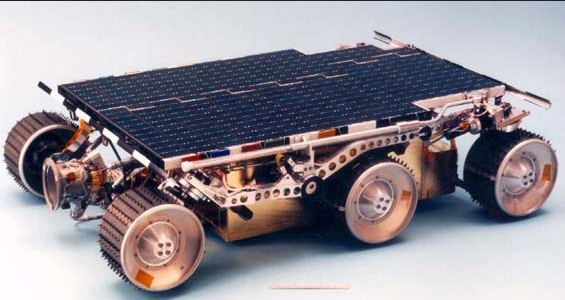
\includegraphics[scale=0.6]{figuras/nasa.png}
 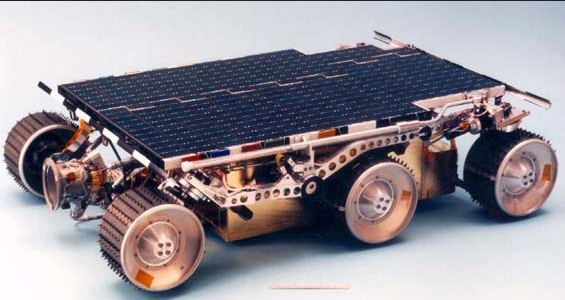
\includegraphics[scale=0.4]{figuras/nasa.png}
 \caption{Veículo exploratório Sojourner \label{fig:nasa}}
 \vspace{-0.3cm}
 \caption*{Fonte: \cite{nasarover}}
\end{figure}


A robótica móvel lida com o controle de veículos autônomos e semi-autônomos, tendo ênfase em problemas relacionados com o 
espaço em larga escala, que são regiões com espaços consideravelmente maiores que as observáveis pelo ponto de visão 
do robô. O espaço em larga escala é de extrema importância para um robô móvel, visto que afeta 
o seu movimento, compreensão e raciocínio nesta área, sendo estes três subproblemas essenciais para este campo de pesquisa
\cite{dudek_mobile}.


\begin{comment}
% Retirado do livro do dudek
A mobile robot is a combination of various physical (hardware) and computational (soft-
ware) components. In terms of hardware components, a mobile robot can be considered
as a collection of subsystems for:
Locomotion: How the robot moves through its environment
Sensing: How the robot measures properties of itself and its environment
Reasoning: How the robot maps these measurements into actions
Communication: How the robot communicates with an outside operator
Later chapters consider the algorithms and representations that make these capabilities
possible, while this chapter concentrates on the underlying hardware, with special empha-
sis on locomotion for wheeled robots.
\end{comment}


%  No mean feat, this makes
%mobile robotics as interdisciplinary a field as there can be. To solve locomotion problems,
%the mobile roboticist must understand mechanism and kinematics, dynamics and control
%theory. To create robust perceptual systems, the mobile roboticist must leverage the fields
%of signal analysis and specialized bodies of knowledge such as computer vision to properly
%employ a multitude of sensor technologies. Localization and navigation demand knowl-
%edge of computer algorithms, information theory, artificial intelligence, a
  
\citeonline{Intro_auto} classifica os robôs móveis em duas categorias relacionadas à locomoção: 
\begin{itemize}
 
 \item Robôs terrestres (\textit{legged robots}): Tem como vantagem a manipulação de objetos e a locomoção em terrenos 
acidentados, mas tem alta complexidade mecânica e energética. A Figura \ref{fig:boston} mostra o 
\textit{Legged Squad Support Systems} (\sigla{LS3}{\textit{Legged Squad Support Systems}}) da Boston Dynamics, 
projetado para atuar nos mesmos terrenos acidentados utilizados por \textit{marines} e soldados norte-americanos, 
ajudando a carregar equipamentos \cite{bostondyn}. 
\begin{figure}[h]
 \centering
 \captionsetup{width=0.44\textwidth,font=footnotesize,textfont=bf}
 %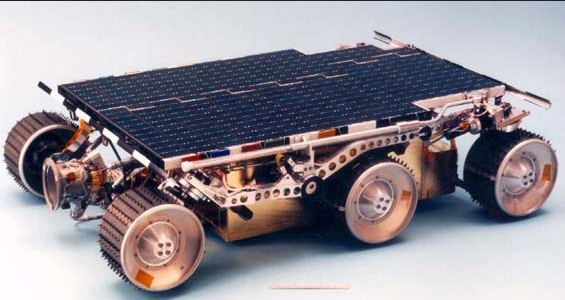
\includegraphics[scale=0.6]{figuras/nasa.png}
 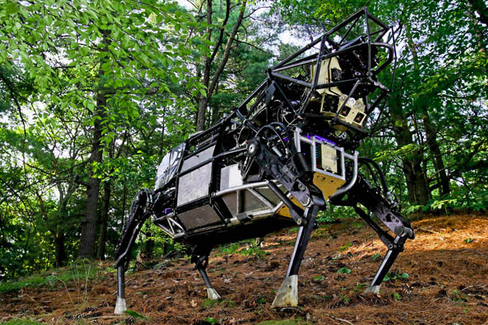
\includegraphics[scale=0.4]{figuras/bostondyn.png}
 \caption{Robô terrestre  L3S\label{fig:boston}}
 \vspace{-0.3cm}
 \caption*{Fonte: \cite{bostondyn}}
\end{figure}


\item Robôs com rodas (\textit{wheeled robots}): É o tipo de locomoção mais utilizado em robôs móveis e veículos. Normalmente o 
equilíbrio não é levado em consideração, visto que na maior parte dos projetos as rodas são consideradas em contato com o solo 
o tempo todo. O robô Sojourner da Figura \ref{fig:nasa} é um exemplo de robô com rodas.%\par
\end{itemize}

\begin{comment}

%%%%%%%%%%%%%%%%%%%%%%%%%%%%%%%%%%%%%%%%%%%%%%%%%%%%%%%%%%%%%%%%%%%%%%%%%%%%%%%%%%%%%%%%%%%%%%%%%%%%%%%%%%%%%%%%%%%%%%%%%%%%%
%%% 	ESTA PARTE VAI NO FINAL COMO TRABALHOS RELACIONADOS

%% Na revisão bibliográfica a seguir são mostradas técnicas desenvolvidas para o sistema de navegação de robôs móveis autônomos.


%\citeonline{ufrj} propôs o desenvolvimento de uma arquitetura híbrida
% ufrj -> Dissertação da UFRJ
O objetivo do trabalho de \citeonline{ufrj} foi o desenvolvimento de um sistema robótico autônomo em uma 
arquitetura híbrida de três camadas, composta pela implementação das camadas Planejador e Executivo. 
%O estudo de caso foi feito pela sistema robótico DORIS, um robô \textit{offshore} (no mar a uma certa distância 
%da orla) guiado por trilhos, 
O estudo de caso foi feito pela sistema robótico DORIS, um robô \textit{offshore}\footnote{\textit{offshore} 
significa estar afastado da costa; em alto mar.} 
%\footnotetext{\textit{offshore} é quando algo está localizado no mar, a uma certa distância 
%da costa (MELHORAR SIGNIFICADO)}
guiado por trilhos, desenvolvido pela COPPE/\sigla{UFRJ}{Universidade Federal do Rio de Janeiro}, 
em parceria com a Petrobras e a Statoil, para a inspeção de plataformas de petróleo. O veículo 
tem como funcionalidades a detecção de anomalias por vídeo, áudio, vibração, temperatura e por câmera de infravermelho e o 
mapeamento 3D do ambiente.


\citeonline{heinen} também propôs uma arquitetura de controle híbrida, integrando as técnicas de controle deliberativo e 
reativo em uma abordagem de três camadas: Deliberativa, a qual determina um trajeto até o objetivo e evita colisões com obstáculos 
já conhecidos, Vital, que utiliza de comportamentos reativos para guiar o robô ao seu objetivo e evitar colisões com obstáculos 
(sejam estes estáticos ou dinâmicos), e Funcional, que faz a integração das camadas vital e deliberativa, fornecendo parâmetros 
reativos para a camada vital. O sistema de controle proposto foi implementado no simulador SimRob3D, o qual permite a utilização de 
modelos de ambiente 
tridimensionais, assim como sensoriais e cinemáticos, permitindo que estes possam ser alterados em tempo real.


A pesquisa de \citeonline{pessin} se concentra na busca por soluções inteligentes aplicadas em robôs móveis autônomos visando a operação 
destes em ambientes dinâmicos. Através da aplicação de aprendizado de máquina, buscou-se uma nova visão sobre a operação destes 
dispositivos em três desafios da área: navegação, localização e operações com grupos de robôs. 
No estudo das operações com grupos de robôs, foi utilizada uma aplicação de combate a 
incêndios, com a avaliação por quatro técnicas: Algoritmos Genéticos, 
Otimização por Enxame de Partículas, \textit{Hill Climbing} e \textit{Simulated Annealing}. Na investigação sobre a navegação, é 
apresentado o desenvolvimento de um veículo autônomo de grande porte, funcional para ambientes externos. Relacionado com a localização, 
é mostrado um método que provê informações de localização para os robôs com base em dados obtidos por redes sem fio.



Nas Figuras \ref{fig:marcio}, \ref{fig:pololu} e \ref{fig:allan} são mostrados os dois protótipos desenvolvidos por \citeonline{alemao} e 
o de \citeonline{allan}, respectivamente, os quais já foram discutidos anteriormente. Na Figura \ref{fig:hirai} é mostrado o 
Cartisx04, robô seguidor de linha de \citeonline{Hirai}, um dos melhores do segmento mundialmente. 
Estes veículos irão fomentar a base de conhecimento deste trabalho.



\begin{figure}[h]
    \centering
    \captionsetup{width=0.83\textwidth,font=footnotesize,textfont=bf}
    \begin{subfigure}[b]{0.4\textwidth}
        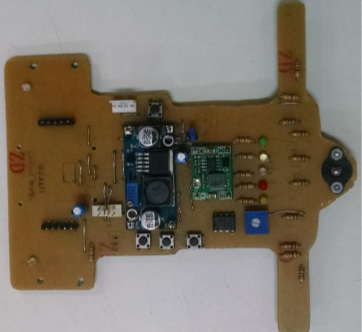
\includegraphics[width=\textwidth,height=0.18\textheight]{figuras/marcio1.png}
        \caption{\centering \label{fig:marcio}}
    \end{subfigure}
    ~ %add desired spacing between images, e. g. ~, \quad, \qquad, \hfill etc. 
      %(or a blank line to force the subfigure onto a new line)
    \begin{subfigure}[b]{0.4\textwidth}
	\centering
        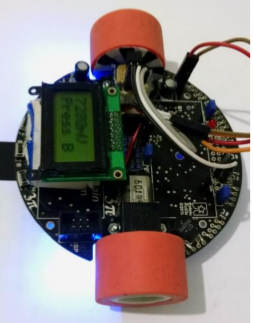
\includegraphics[width=0.75\textwidth,height=0.18\textheight]{figuras/polulumod.png}
        \caption{\centering \label{fig:pololu}}
    \end{subfigure}
    
    \begin{subfigure}[b]{0.4\textwidth}
        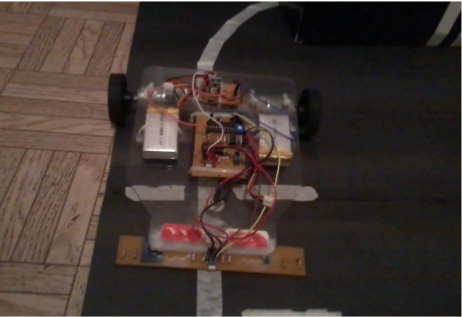
\includegraphics[width=\textwidth,height=0.18\textheight]{figuras/allan.png}
        \caption{\centering \label{fig:allan}}
    \end{subfigure}
    % THE CAPTION PREVIOUSLY WAS HERE
    ~ %add desired spacing between images, e. g. ~, \quad, \qquad, \hfill etc. 
      %(or a blank line to force the subfigure onto a new line)
    \begin{subfigure}[b]{0.4\textwidth}
        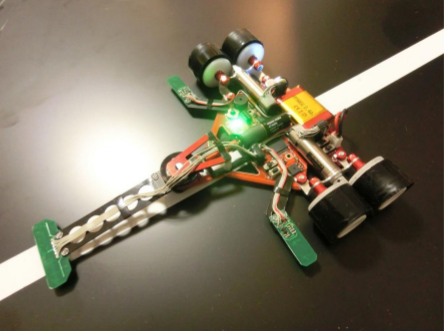
\includegraphics[width=\textwidth,height=0.18\textheight]{figuras/Hirai.png}
        \caption{\centering \label{fig:hirai}}
    \end{subfigure}
    
    \caption{\label{fig:segLinha} Robôs seguidores de linha: (a) Robô \textit{Alpha Project} \cite{alemao}; 
    (b) Pololu 3pi modificado \cite{alemao}; (c) Protótipo de \citeonline{allan}; (d) Cartisx04 de \citeonline{Hirai}.}
\end{figure}

%%%%%%%%%%%%%%%%%%%%%%%%%%%%%%%%%%%%%% END OF FILE %%%%%%%%%%%%%%%%%%%%%%%%%%%%%%%%%%%%%%%%%%%%%%%%%

\end{comment}




\begin{comment}
		  TENTAR APROVEITAR ESTA PARTE!
%%%%%%%%%%%%%%%%%%%%%%%%%%%%%%%%%%%%%%%%%%%%%%%%%%%%%%%%%%%%%%%%%%%%%%%%%%%%%%%%%%%%%%%%%%%%%%%%%%%%%%%%%%%%%%%%%%%%%%%%%%
\vspace{1cm}
\section{Sistema embarcado}

Por mais que apresentem ser invisíveis, ....


%Segundo Li e Qual (sei lá? 2008), um sistema embarcado é \textit{Um sistema embarcado é um sistema BLABLABLA... continua}.
Sistemas embarcados são sistemas computacionais que integram \textit{harware} e \textit{software}, com o objetivo de 
rodar uma aplicação específica \cite{embedded}. Os sistemas embarcados são encontrados na forma de circuitos integrados 
\sigla{CI}{Circuitos Integrados}, o que possibilita que estes dispositivos tenham uma grande quantidade de aplicações (Melhorar ?). 

Os sistemas embarcados podem ser separados em duas categorias: Os de lógica reconfigurável e os sistemas microcontrolados.
xxxxxxxxxxxxxxxxxxx



Para (Stallings-arquitetura), o termo sistema embarcado combina de \textit{hardware} e \texit{software} de computador (fjdslfsjdj)


\subsection{Microcontroladores}

Os microcontroladores são dispositivos xxxxx (referenciar alguém).
São compostos por CPU, ADC xxxxxxxx xxxxxx.

\end{comment}



%%%%%%%%%%%%%%%%%%%%%%%%%%%%%%%%%%%%%%%%%%%%%%%%%%%%%%%%%%%%%%%%%%%%%%%%%%%%%%%%%%%%%%%%%%%%%%%%%%%%%%%%%%%%%%%%%%%%%%%%%%%
\vspace{1cm}
\section{Sistemas de Controle para robôs móveis} \label{cap:controle}

Para que o robô seja autônomo, 
é necessário que este apresente uma resposta desejada para 
as mais diversas situações. 
Para tanto se utiliza de um sistema de controle, que consiste em subsistemas e processos, conhecidos como plantas, 
dos quais se obtém uma saída com desempenho desejado para uma dada entrada \cite{nise}. Na Figura 
\ref{fig:basicdiag} é mostrado o diagrama de blocos\footnote{Diagrama de blocos é uma representação gráfica do sistema que mostra o 
fluxo de sinais que ocorre entre os componentes deste.} de 
um sistema de controle em uma forma simplificada, em que aplicando-se uma entrada a este, obtêm-se uma 
resposta. 

\begin{figure}[h]
 \centering
 \captionsetup{width=0.6\textwidth,font=footnotesize,textfont=bf}
 %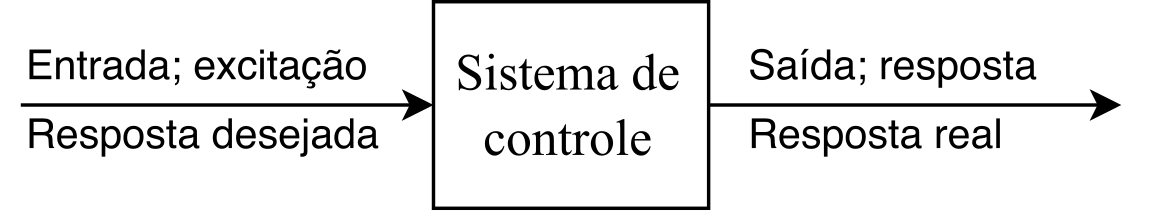
\includegraphics[width=0.6\textwidth]{figuras/DiagramaNise.png}
 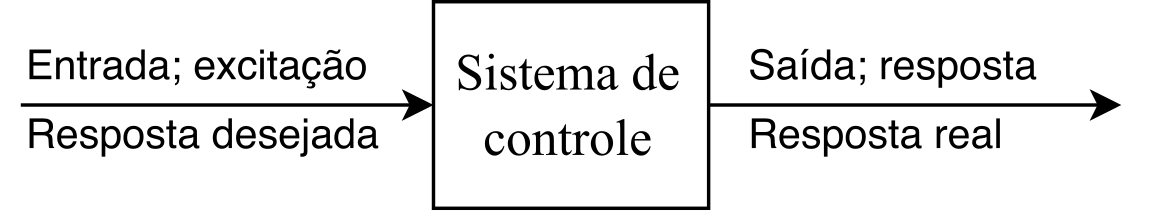
\includegraphics[width=0.6\textwidth]{figuras/DiagramaNise.png}
 \caption{Descrição de um sistema de controle \label{fig:basicdiag}}
  \vspace{-0.3cm}
 \caption*{Fonte: Adaptado de \cite[p.2]{nise}.}
\end{figure}


\begin{comment}
Segundo \citeonline{Intro_auto}, o controle de movimento de 
um sistema não-holomônico\footnote{Sistemas não-holomônicos são sistemas não integráveis} não é trivial, no entanto estão disponíveis 
soluções adequadas para contornar este contratempo:
\begin{itemize}
 \item Controle por malha aberta (\textit{Open loop control}): Não utiliza de sensores, logo o veículo segue uma trajetória descrita por 
 sua posição e velocidade como uma função de tempo e a sua posição não retorna (\textit{feedback}) para o controle da velocidade e 
 controle. Mesmo sendo de mais fácil implementação, apresenta várias restrições, como a impossibilidade de se adaptar 
 automaticamente ao ambiente caso aconteçam mudanças dinâmicas neste.
 \item Controle por Malha fechada (\textit{Closed loop control}): É uma abordagem mais apropriada para o controle de movimento, visto que 
os sensores são continuamente monitorados e os atuadores\footnote{Atuadores são dispositivos capazes de alterar 
o estado do sistema controlado com base em sinais de controle, como por exemplo os motores elétricos.} são ajustados com base nestes 
valores \cite{heinen}. 
\end{itemize}
\end{comment}

Para \citeonline{nise} os sistemas de controle podem ser classificados em duas configurações principais:
\begin{itemize}
 \item Controle por malha aberta (\textit{Open loop control}): É a configuração mais simples, onde o sinal 
 de saída não exerce nenhuma ação de controle no sistema \cite{ogata}. Desta forma, um sistema de controle de malha aberta 
 não é medido e nem comparado com a entrada, como pode ser visto na Figura \ref{fig:Malhaaberta}, não sendo capaz de compensar 
 distúrbios que possam ser adicionados ao sistema \cite{nise}.
 
 \item Controle por Malha fechada (\textit{Closed loop control}): Nesta configuração, a saída ou a resposta influencia a entrada do 
 sistema \cite{controle}. Logo após a Resposta Desejada, na Figura \ref{fig:Malhafechada}, tem-se um ponto de soma, em que será feita 
 a soma algébrica dos sinais associados. % \citeonline{nise} diz que
 %este ponto de soma adiciona o sinal da entrada (também conhecido como referência) ao sinal 
 %da saída do sistema, o qual chega através de um caminho de retorno (\textit{feedback path}). 
 %
 %O erro do sistema é obtido subtraindo-se o 
 %sinal de saída pelo de entrada do sistema. Esta configuração permite que sejam compensados distúrbios no sistema, visto que se caso haja 
 %divergência entre as duas respostas, o sistema aciona a planta pelo erro
 Segundo \citeonline{ogata}, o sinal de erro atuante, que é a diferença entre o sinal de entrada e o sinal de realimentação (o qual é 
 calculado logo após o ponto de soma, como pode ser visto na Figura \ref{fig:controlador}), 
 realimenta o controlador que tende a minimizar o erro e deixar a saída com o valor desejado.
\end{itemize}


\begin{figure}[h]
    \centering
    \captionsetup{width=0.8\textwidth,font=footnotesize,textfont=bf}
    \begin{subfigure}[b]{0.8\textwidth}
	\centering
        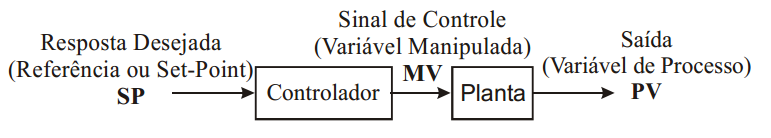
\includegraphics[width=\textwidth,height=\textheight,keepaspectratio]{figuras/MalhaAberta.png}
        \caption{\centering \label{fig:Malhaaberta}}
    \end{subfigure}
    %~ 
    
    \begin{subfigure}[b]{0.8\textwidth}
	\centering
        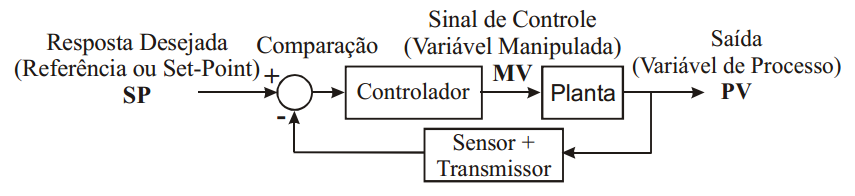
\includegraphics[width=\textwidth,height=\textheight,keepaspectratio]{figuras/MalhaFechada.png}
        \caption{\centering \label{fig:Malhafechada}}
    \end{subfigure}
    
    %\caption{\label{fig:Malhas} Técnicas de controle: (a) Malha aberta; (b) Malha fechada \cite{Intro_auto}} 
    \caption{\label{fig:Malhas} Configurações de sistemas de controle: (a) Malha aberta; (b) Malha fechada \cite{controle}} 
\end{figure}


\subsection{Ações de controle}

Conforme \citeonline{ogata}, um controlador automático compara o valor de saída da planta com a entrada do sistema, 
determinando o desvio e produzindo um sinal de controle que reduzirá este desvio a um valor pequeno. É chamada de ação de controle a 
maneira pela qual o controlador produz o sinal de controle. Na Figura \ref{fig:controlador} é mostrado o diagrama de blocos 
de um sistema de controle, composto por um controlador automático, um atuador, uma planta e um sensor, o qual é 
o elemento de medição. Os atuadores são dispositivos capazes de alterar 
o estado do sistema controlado com base em sinais de controle, como os motores elétricos. O sensor é um elemento que 
converte a variável de saída em uma outra variável pertinente, que possa ser mensurável pelo sistema.

\begin{figure}[h!]
 \centering
 \captionsetup{width=0.8\textwidth,font=footnotesize,textfont=bf}
 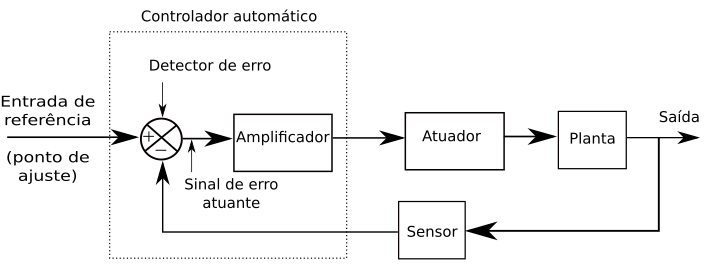
\includegraphics[width=0.8\textwidth,height=0.5\textheight,keepaspectratio]{figuras/Controlador.png}
 \caption{Diagrama de blocos de um controlador automático \label{fig:controlador}}
 \vspace{-0.2cm}
 \caption*{Fonte: Adaptado de \cite[p.18]{ogata}.}
\end{figure}

\citeonline{ogata} classifica os controladores industriais de acordo com as suas ações de controle:
\begin{itemize}
 \item Controlador de duas posições ou \textit{on-off}; %(OBS.: TALVEZ DE PROBLEMA NESSE TEXTIT ANTERIOR)
 \item Controlador Proporcional;
 \item Controlador Integral;
 \item Controlador Proporcional-Integral (\sigla{PI}{Proporcional-Integral});
 \item Controlador Proporcional-Derivativo (\sigla{PD}{Proporcional-Derivativo});
 \item Controlador Proporcional-Integral-Derivativo (\sigla{PID}{Proporcional-Integral-Derivativo})
\end{itemize}

\subsubsection{Controlador \textit{on-off}}

Em controladores de duas posições ou \textit{on-off}, o elemento atuante tem somente duas posições, as quais são fixas, geralmente sendo 
\textit{on} (ligado) e \textit{off} (desligado) \cite{ogata}. Tem grande aplicabilidade em sistemas de controle industriais e 
domésticos, devido ao baixo custo e simplicidade de implementação.

Considerando-se o sinal de saída do controlador $u(t)$ % $ é indicativo para equação
e o sinal de erro atuante $e(t)$, o sinal $u(t)$ apresenta um valor máximo ou mínimo, caso o erro atuante seja negativo ou positivo, 
respectivamente. Assim, tem-se que:

%begin{align*}  %%Utiliza-se o align quando não deseja ter numeração nas equações
% u(t) = U_1, \quad para \ e(t) \ > \ 0, \\
% u(t) = U_2, \quad para \ e(t) \ < \ 0,
%\end{align*}

\begin{equation}
 u(t) = U_1, \quad para \ e(t) \ > \ 0, \\ 
\end{equation}
\begin{equation}
 u(t) = U_2, \quad para \ e(t) \ < \ 0,
\end{equation}

em que $U_1$ e $U_2$ são constantes.
Em problemas de controle mais complexos, se faz necessária a utilização de outros controladores, devido ao \textit{on-off} apresentar 
muitas oscilações e \textit{offset}\footnote{\textit{Offset} é um erro entre o valor desejado e o valor obtido.}.

s defined as the voltage that must be applied between the two input
terminals of the op amp to obtain zero volts at the output. Ideally the output of the op amp should
be at zero volts when the inputs are grounded. 

\subsubsection{Controlador Proporcional}


Na ação de controle proporcional, a relação entre a saída do controlador $u(t)$ e o sinal de erro $e(t)$ 
é apenas um ganho: 
%A equação \ref{eq:prop} mostra a equação do controlador proporcional.

\begin{equation}\label{eq:prop}
 u(t) = K_pe(t),	
\end{equation}
em que $K_p$ é o ganho do controlador proporcional. 
Para \citeonline{controle} quanto maior o ganho, menor será o erro $e(t)$, no entanto o sistema pode perder estabilidade 
devido ao aumento do 
tempo de acomodação\footnote{Tempo de acomodação (\textit{settling time}) é o tempo para que a curva de resposta alcance 
valores em uma faixa (2\% a 5\%) em relação ao valor final, permanecendo nesta faixa interminavelmente.}.

\subsubsection{Controlador Integral}

Segundo \citeonline{ogata}, na ação de controle integral, o valor da saída $u(t)$ é alterado a uma taxa de variação proporcional 
ao sinal de erro atuante $e(t)$:

\begin{equation}
 %u(t) = K_i \int_{lower}^{upper}
 u(t) = K_i \int_{0}^{t}e(t)dt,
\end{equation}

em que $K_i$ é a constante de ganho integral. 

\subsubsection{Controlador Proporcional-Integral (PI)}

Para \citeonline{nise}, um controlador Proporcional-Integral pode ser chamado de compensador integral ideal, visto que 
as ações de controle Proporcional e Integral alimentam o erro e a integral do erro para a planta, respectivamente, desta forma 
tendendo a eliminar o erro em regime permanente\footnote{A resposta temporal de um sistema consiste em duas 
partes: da resposta transitória e da resposta estacionária ou em regime permanente}. 
A sua ação de controle é definida por: 

\begin{equation}
 u(t) = K_pe(t) + \frac{K_p}{T_i}\int_{0}^{t}e(t)dt,
\end{equation}
em que $T_i$ é chamado de tempo integrativo. 


\subsubsection{Controlador Proporcional-Derivativo (PD)}

%\citeonline{nise} denomina o controlador Proporcional-Derivativo um compensador derivativo ideal, o qual compreende as 
%ações proporcional, consistindo na alimentação do erro, e derivativa, a qual é proporcional à derivada do erro. 

Segundo \citeonline{controle}, as ações proporcional e derivativa deste controlador 
contribuem com o regime transitório, %\footnote{A resposta transitória de um sistema é aquela que vai do estado inicial ao final}, 
tendendo a aumentar a estabilidade do sistema e reduzir o tempo de acomodação. 
A ação de controle deste controlador é definida por:
\begin{equation}
 u(t) = K_pe(t) + K_pT_d\frac{de(t)}{dt}
\end{equation}
em que $T_d$ é chamado de tempo derivativo \cite{ogata}.


\subsubsection{Controlador Proporcional-Integral-Derivativo (PID)}

O controlador Proporcional-Integral-Derivativo reúne a ação das três ações de controle, atuando na melhoria do 
regime permanente e da resposta transitória. 
A equação do controlador é dada por:

\begin{equation}
 u(t) = K_pe(t) + \frac{K_p}{T_i}\int_{0}^{t}e(t)dt + K_pT_d\frac{de(t)}{dt}
\end{equation}
em que  $K_p$ é o ganho proporcional, $T_i$ é o tempo integrativo e $T_d$ é o tempo derivativo \cite{ogata}.


%%%%%%
%
%  Este aqui ta bacana:
%  http://www.dca.ufrn.br/~meneghet/FTP/Controle/scv20071.pdf
%
%%%%%%


%%%%%%%%%%%%%%%%%%%%%%%%%%%%%%%%%%%%%%%%%%%%%%%%%%%%%%%%%%%%%%%%%%%%%%%%%%%%%%%%%%%%%%%%%%%%%%%%%%%%%%%%%%%%%%%%%%%%%%%%%%%
\vspace{1cm}
\section{Sistemas a Eventos Discretos} \label{cap:sed}

%O sistema de controle híbrido a ser implementado é composto pelo sistema de controle discreto, 
%Os sistemas podem ser classificados em relação à natureza do espaço de estados selecionado, podendo ser 

Para \citeonline{cassandras}, os sistemas podem ser classificados em duas categorias quanto à natureza do espaço de estados 
selecionado: 
\begin{itemize}
 \item Estado contínuo: O espaço de estados $X$ é uma continuidade, compreendendo todos os vetores $n$-dimensionais de números reais ou 
 complexos, eventualmente;
 
 \item Estado discreto: O espaço de estados é um conjunto discreto. As variáveis de estado deslocam-se em pontos discretos no tempo, de 
 um valor estado discreto para outro.
\end{itemize}

\citeonline{teixeira} diz que a modelagem computacional de um sistema pode ser estruturada em dois fundamentos:
\begin{itemize}
 \item Estado, que determina o \textit{status} do sistema em determinada situação;
 %\item Noção de estado, que determina o \textit{status} do sistema em determinada situação;
 %Teixeira, Pg 37
 \item Transição de estados, o qual caracteriza o crescimento do sistema.
 %\item Técnica de transição de estados, o qual caracteriza o crescimento do sistema.
\end{itemize}

Alguns sistemas são mapeados continuamente e suas estruturas de transição são regidas pelo tempo, 
enquanto que em outros sistemas seus estados podem não ser contínuos e as transições não dependem do tempo, mas de 
eventos instantâneos e assíncronos, como o processamento de um dado em um equipamento computacional, em que o conjunto de estados é 
discreto e as transições não são feitas por tempo, mas por eventos como \textit{clock} e interrupções 
\cite{teixeira}. 
%No exemplo apresentado por \citeonline{teixeira}, do processamento de dado em algum 
%equipamento computacional, em que o conjunto 

%Segundo \citeonline{teixeira}, 
%alguns sistemas são mapeados continuamente e suas estruturas de transição são regidas pelo tempo, sendo geralmente modelados através de 
%equações diferenciais. Em outros sistemas, em que o espaço de estados pode não ser contínuo e as transições de estados não dependa de 
%tempo, mas de eventos instantâneos e assíncronos, a modelagem por equações diferenciais pode não ser a mais conveniente. 

\citeonline{torrico} define um Sistema a Eventos Discretos (\sigla{SED}{Sistema a Eventos Discretos}) 
como um sistema dinâmico a estado discreto que evolui à proporção assíncrona de eventos. 
Deste modo, os SEDs tem como características o espaço de estados ser discreto e o mecanismo de transição de estados ser 
dirigido por eventos.

Alguns exemplos dos Sistemas a Eventos Discretos, conforme \citeonline{cassandras}, são os Sistemas de Filas, os Sistemas 
de Computador, Sistemas de Comunicação e Sistemas de Manufatura. 

%\subsection{Modelagem do SED}
\subsection{Linguagens e Autômatos}


Uma das maneiras formais de se estudar o comportamento lógico de um SED é baseado nas teorias de linguagens e autômatos, que se dá pelo 
fato de qualquer Sistema a Eventos Discretos ter um conjunto implícito $E$ associado a ele. \citeonline{cassandras} chama esse 
conjunto $E$ e a sequência de eventos como 
\textquotedblleft alfabeto\textquotedblright e \textquotedblleft palavras\textquotedblright de linguagem, respectivamente. Para 
demonstrar estes conceitos, o autor fala do exemplo de uma máquina que é ligada uma ou duas vezes ao dia, como um carro ou um computador 
pessoal, e deseja-se projetar um sistema que realize uma simples tarefa: Quando a máquina estiver ligada, esta primeiramente deve 
indicar que está ligada e depois reportar este fato (como \textquotedblleft checar óleo\textquotedblright, caso seja um 
carro). Neste caso, cada um destes sinais define um evento, enquanto que todos os sinais possíveis que a máquina possa emitir são 
definidos como uma sequência de eventos, ou alfabeto.

%\citeonline{teixeira} define um Autônomo Finito (\sigla{AF}{Autônomo Finito}) como uma estrutura formal de 
\citeonline{cassandras} define um autômato como um dispositivo apropriado para representar a linguagem de acordo com regras bem 
definidas. Caso o conjunto de estados do autômato seja finito e caso este seja determinístico, ou seja, que este não possua 
duas ou mais transições com o mesmo nome saindo de um estado, o autômato é chamado de Autômato Finito Determinístico 
(\sigla{AFD}{Autômato Finito Determinístico}). \citeonline{torrico} diz que um autômato pode ser representado por uma tabela ou 
por um diagrama de transição de estados, sendo que neste os estados e as transições 
da máquina podem ser representados por vértices do diagrama e por arcos que conectam estes vértices, respectivamente.
Duas variantes dos autômatos são os Autômatos de Mealy e de Moore, as quais serão clarificadas a seguir.
%Duas variantes dos autômatos são:
%Os autômatos podem ser divididos em duas variações, as quais são:


\subsubsection{Autômato de Moore}

O modelo de Moore são autômatos com saídas de estados, em que há uma função de saída a qual especifica uma saída para cada estado 
\cite{cassandras}. %As transições não possuem funções de saída, as quais neste caso estão associadas aos eventos. 
%A saída depende somente do estado atual. 
As ações são produzidas nos estados e a saída depende somente do estado atual. 
Um exemplo do Autômato de Moore pode ser visto na Figura \ref{fig:Moore}, em que a saída associada a cada estado é 
mostrada em negrito (cada saída é acionada pelo autômato quando este entra no estado).

\begin{figure}[h!]
 \centering
 \captionsetup{width=0.5\textwidth,font=footnotesize,textfont=bf}
 %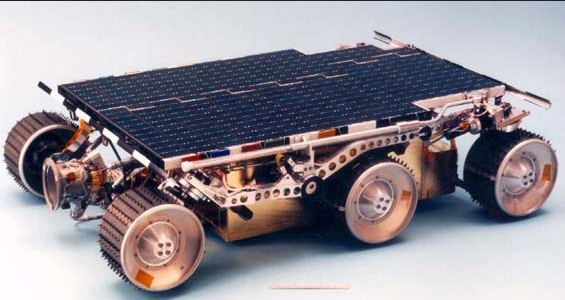
\includegraphics[scale=0.6]{figuras/nasa.png}
 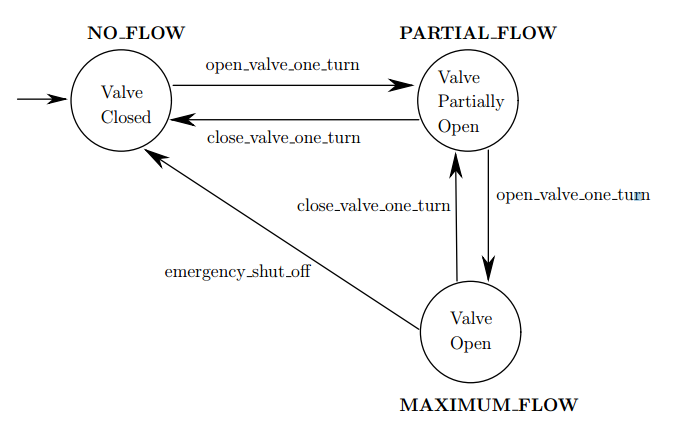
\includegraphics[scale=0.4]{figuras/moore.png}
 \caption{Autômato de Moore \label{fig:Moore}}
 \vspace{-0.3cm}
 \caption*{Fonte: \cite[p.73]{cassandras}}
\end{figure}

\subsubsection{Autômato de Mealy} 
\begin{comment}
O modelo de Mealy são autômatos de entrada e saída, em que as transições são denominadas por \textquotedblleft eventos\textquotedblright 
na forma de eventos de entrada e saída \cite{cassandras}.

produz um resultado (saída de dados) baseando-se no estado em que se encontra e na entrada de dados. Isto significa que o 
diagrama de estados irá incluir tanto o sinal de entrada como o de saída para cada vértice de transição.

Já   a   Máquina   de   Mealy   é   um   
Autômato  Finito  modificado  de  forma  a  
gerar  uma  palavra  de  saída  para  cada  
transição 
entre os estados.

Em uma máquina de Mealy a saída depende da entrada e do estado, representando a evolução de
estados, numa sequência. Uma transição tem uma ação de saída e qualquer ação de saída pode ser
usada em mais de uma transição. Ações de saída não são associadas a estados, que são passivos.
Neste caso, as ações de saída podem ser associadas a mais de um estado.
\end{comment}
Diferentemente de Moore, o autômato de Mealy depende da entrada e da saída do estado, representando 
sequencialmente o crescimento dos estados. Conforme mostra a Figura \ref{fig:Mealy}, as funções de saída estão nas transições. 
Este modelo funciona da seguinte maneira para uma transição $e_i/e_o$ do estado $x$ para o estado $y$: Quando o sistema estiver no 
estado $x$, o autômato receberá o evento de entrada $e_i$ e expedirá o evento de saída $e_o$ durante a transição para $y$ 
\cite{cassandras}.



\begin{figure}[h!]
 \centering
 \captionsetup{width=0.5\textwidth,font=footnotesize,textfont=bf}
 %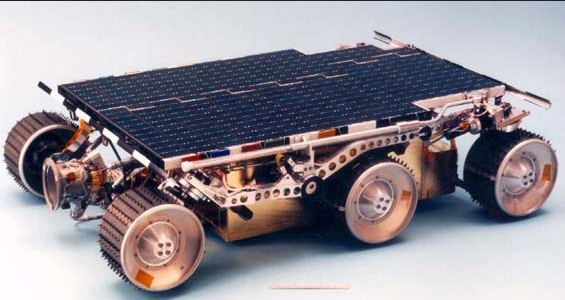
\includegraphics[scale=0.6]{figuras/nasa.png}
 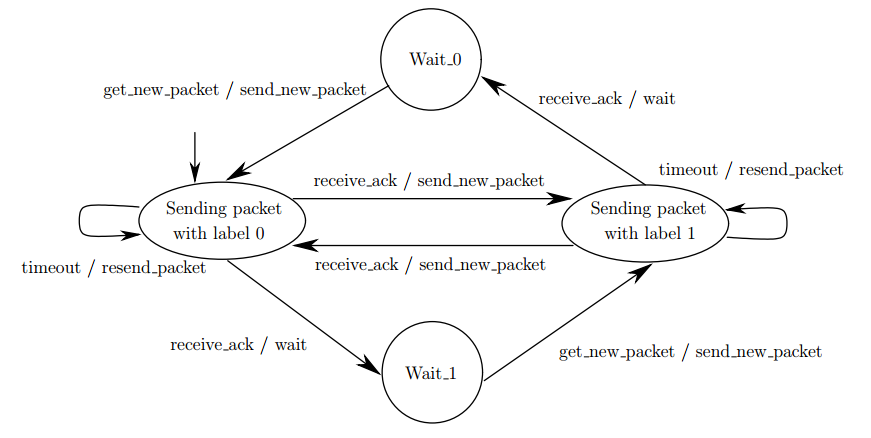
\includegraphics[scale=0.4]{figuras/mealy.png}
 \caption{Autômato de Mealy \label{fig:Mealy}}
 \vspace{-0.3cm}
 \caption*{Fonte: \cite[p.73]{cassandras}}
\end{figure}

\begin{comment}


\begin{itemize}
 \item Autômato de Moore (autômatos com saídas): Neste modelo, 
há uma função de saída que garante uma saída para cada estado \cite{cassandras}. As transições não apresentam uma ação de saída.
Um exemplo pode ser visto na Figura \ref{fig:Moore}, em que a saída associada a cada 
estado é mostrada em negrito.
 \item Autômato de Mealy (autômatos de entrada e saída): As transições são nomeadas por eventos da forma de entrada e saída... 
A saída depende do valor da entrada e do estado, reproduzindo sequencialmente a evolução dos estados. As ações de saída são 
associadas %%%%%
Em uma máquina de Mealy a saída depende da entrada e do estado, representando a evolução de
estados, numa sequência. Uma transição tem uma ação de saída e qualquer ação de saída pode ser
usada em mais de uma transição. Ações de saída não são associadas a estados, que são passivos.
Neste caso, as ações de saída podem ser associadas a mais de um estado.
A Figura abaixo apresenta uma máquina de Mealy. Observe que os valores de entrada (input)
resultam em valores na saída (output). Inicialmente, a máquina inicia no estado 0 (estado inicial). Ao entrar
um caractere ‘a’, ocorre uma transição do estado 0 para o estado 1, sendo que na transição a ação, ou
seja, a saída é definida como sendo 0. Na sequencia, um novo caractere ‘a’ entra e provoca uma transição
do estado 1 para o estado 3, gerando uma saída igual a 1, e assim por diante.
 %%%%%%%%%%%%%%%%%%%%%%
\end{itemize}
\end{comment}
 
%\subsubsection{Autômato de Moore} 
%\subsubsection{Autômato de Mealy} 



%%%%%%%%%%%%%%%%%%%%%%%%%%%%%%%%%%%%%%%%%%%%%%%%%%%%%%%%%%%%%%%%%%%%%%%%%%%%%%%%%%%%%%%%%%%%%%%%%%%%%%%%%%%%%%%%%%%%%%%%%%%
%\vspace{1cm}
\vspace{2cm} %% VERIFICAR MELHOR ISTO AQUI DEPOIS
%\section{Sensores para robôs móveis} \label{cap:sensores}
%\section{Sensores e atuadores} \label{cap:sensores}
\section{Estrutura de um robô móvel} \label{cap:sensores}

%Conforme \citeonline{dudek_mobile}, para que um robô possa 
%\citeonline{dudek_mobile} diz que para um robô deve ser capaz de mover e sentir


%O controle de malha fechada, o qual foi abordado anteriormente, necessariamente precisa do sinal de sensores para realizar o 
%\textit{feedback} (realimentação) do sistema. 
%Em vista disso, esta seção se preocupa com os sensores e atuadores necessários para o projeto de um robô móvel.\par

%\citeonline{dudek_mobile} diz que os robôs podem ser divididos em 
%\textit{hardware} e \textit{software}, os quais representam, nesta ordem, os componentes físicos e computacionais da máquina. 
%O autor classifica 
%Em 
%relação aos componentes de \textit{hardware} do dispositivo, o autor classifica da seguinte forma:
\citeonline{dudek_mobile} classifica os componentes físicos (\textit{hardware}) dos robôs móveis em quatro partes:

\begin{itemize}
 \item Locomoção: É como o robô se move pelo ambiente; 
 
 \item Percepção: É como o robô percebe propriedades do ambiente e dele mesmo;
 
 \item Raciocínio: É como o robô transforma a suas medidas em ações;
 
 \item Comunicação: É como que o robô se comunica com um agente externo.
 
\end{itemize}

Com suporte nessa divisão e no restante da literatura, tem-se os seguintes elementos necessários para o projeto de um robô móvel:
%% elementos estava anteriormente como "dispositivos"
\begin{itemize}

%%% BATERIAS 
\item[] \textbf{Bateria}: É um componente essencial do sistema, visto que o robô móvel precisa se locomover pelo espaço e não pode 
ser dependente de uma fonte externa de energia elétrica. \citeonline{dudek_mobile} diz que baterias com bom desempenho e baixo custo são 
as baseadas em células de gel (\textit{gell cell}), 
mas por serem pesadas não são utilizadas com veículos 
leves. Para estes, são utilizadas tecnologias baseadas em Íons de Lítio (\textit{lithium-ion}), 
Níquel-Cádmio (\sigla{NiCad}{Níquel-Cádmio}) e as de Hidreto Metálico de Níquel (\sigla{NiMH}{Hidreto Metálico de Níquel}), as quais são 
originalmente projetadas para serem utilizadas em dispositivos sem-fio, como \textit{laptops} e \textit{smartphones}.

%%%% MOTORES pg 33
\item[] \textbf{Motores}: 
São os responsáveis por fazer com que o veículo \textquotedblleft ande\textquotedblright. 
%, visto que estes convertem energia 
%elétrica em mecânica. Dentre os motores, 
Muitos robôs utilizam a bateria para acionar os motores de passo ou servomotores, os quais convertem energia 
elétrica em mecânica (\citeonline{dudek_mobile}). No entanto existem outros dispositivos, capazes de gerar energia mecânica em movimento, 
como os piezoelétricos e os pneumáticos.\par
\begin{itemize}
 \item O motor de passo (\textit{stepper motor}) é um motor elétrico em que o eixo move uma quantidade contralada a cada pulso, assim, 
controlando estes pulsos obtém-se a saída desejada \cite{dudek_mobile}.\par
 \item O servomotor (\textit{servo motor}) combina um motor elétrico de corrente contínua 
(\sigla{CC}{Corrente Contínua}) ou corrente alternada (\sigla{CA}{Corrente Alternada}) com um sensor de orientação de eixo 
\cite{dudek_mobile}. 
O autor diz ainda que controle dos servomotores é mais complexo que os motores de passo, sendo necessário utilizar um controlador de 
motor mais complexo, os quais variam em complexidade e que geralmente trabalham com parâmetros como posição, velocidade ou 
movimento de saída.
\end{itemize}




%%% SERVO MOTOR CONTROL
\item[] \textbf{Controle de um servomotor}: Podem ser utilizadas as abordagens de malha aberta e malha fechada. No controle 
de malha aberta, o valor desejado do eixo é utilizado para projetar um controlador oportuno, no entanto fica 
suscetível a distúrbios, pois não apresenta realimentação. No controle por malha fechada, a realimentação do sistema é utilizada para 
ajustar o movimento do disposito, sendo que um controlador amplamente utilizado é o PID \cite{dudek_mobile}.

%%% COMUNICAÇÃO
\item[] \textbf{Dispositivo de comunicação}: Devido à necessidade em interagir com um operador humano, como no caso de reportar que 
uma tarefa foi concluída, \citeonline{dudek_mobile} relata que os robôs utilizam de um meio físico para a comunicação, como por cabo, ou 
por comunicação sem-fio (\textit{wireless}), como o \textit{bluetooth} (padrão sem-fio de curto alcance), 802.11 (padrão da IEEE 
\sigla{IEEE}{\textit{Institute of Electrical and Electronics Engineers}} para redes locais sem-fio) ou infravermelho.

%%% PROCESSAMENTO
\item[] \textbf{Processamento}: O processamento é um componente principal dos robôs móveis, tanto que \citeonline{dudek_mobile} 
discute em que lugar o processamento do veículo deve estar. O autor chega na conclusão que a melhor forma do processamento ser feito é 
a de separar as tarefas em \textit{on-board} (dentro do veículo) e \textit{off-board} (fora do veículo), responsáveis, 
respectivamente, pelas tarefas de tempo crítico e as que não são de tempo crítico. Este modelo tem como vantagens a redução no consumo 
de energia do dispositivo.

\item[] \textbf{Sensores}: Os sensores serão abordados na próxima seção.

\end{itemize}

\subsubsection{Sensores não-visuais}

%O controle de malha fechada, o qual foi abordado anteriormente, necessariamente precisa do sinal de sensores para realizar o 
%\textit{feedback} (realimentação) do sistema. 
%Em vista disso, esta seção se preocupa com os sensores e atuadores necessários para o projeto de um robô móvel.\par
\citeonline{secchi2012} diz que os robôs devem ser capazes de realizar três tarefas essenciais: estimar a sua posição e orientação 
(pose), manter o mapa do ambiente atualizado e identificar os possíveis obstáculos deste. %do ambiente.
Desta forma, para que o robô conheça o seu ambiente de trabalho e possa se adaptar a este, é necessário coletar informações e 
adequá-las ao sistema de controle. Assim, O controle de malha fechada, o qual foi abordado anteriormente, 
necessariamente precisa do sinal de sensores para realizar o \textit{feedback} (realimentação) do sistema.\par

\citeonline{dudek_mobile} classifica os sensores em duas variantes: visuais e não-visuais. 
A seguir serão mostrados os principais sensores não-visuais 
dos robôs móveis. Para informações sobre os sensores visuais, consultar \cite{dudek_mobile}, \cite{Intro_auto} e \cite{secchi2012}.

\begin{itemize}
 \item[] \textbf{Sensores inerciais}: São sensores externos que fazem referência com o mundo externo, ou seja, medem variáveis de 
posição do robô.
  \begin{itemize}
   \item Encoder óptico: Estes dispositivos medem a velocidade e a posição angular em um \textit{driver} de motor ou no eixo de uma 
   roda. Este sensor, segundo \citeonline{Intro_auto}, é um interruptor de luz, que produz uma quantidade de pulsos para cada revolução 
   do eixo. Os pulsos gerados pela diferença de fase entre os canais A e B é utilizada determinar a direção de rotação, como pode 
   ser visto na Figura \ref{fig:optical}.
   
   \item Giroscópios: São sensores que preservam a orientação em relação a um referencial fixo, provendo a medida absoluta. Podem ser 
   mecânicos ou ópticos. Na Figura \ref{fig:giro} pode ser visto um giroscópio de dois eixos.
   
   \item Acelerômetros: \citeonline{Intro_auto} diz que estes sensores são capazes de medir todas as forças externas que estejam 
   agindo sobre ele, inclusive a gravidade. 
   São baseados em sistemas pendulares, em que a primeira integração das acelerações proporciona a velocidade e a 
   segunda, a posição \cite{secchi2012}. A precisão deste dispositivo é de grande importância, visto que pequenos erros podem 
   influenciar na posição estimada, devido à dupla integração das acelerações. O diagrama deste dispositivo pode ser visto na Figura 
   \ref{fig:acel}.
  \end{itemize}
  
 \item[] \textbf{Sensores de infravermelho}: São sensores de proximidade rápidos e baratos, que basicamente consistem na emissão de 
 um pulso infravermelho e detecção do sinal refletido, com a distância aproximada calculada através da 
 força do sinal \cite{dudek_mobile}.

\end{itemize}


%\subsubsection{Sensores e atuadores}
%\subsubsection{Sensores e atuadores}


%%%%%%%%%%%%%%%%%%%%%%%%%%%%%%%%%%%%%%%%%%%%%%%%%%%%%%%%%%%%%%%%%%%%%%%%%%%%%%%%%%%%%%%%%%%%%%%%%%%%%%%%%%%%%%%%%%%%%%%%%%%
%\vspace{1cm}
%\section{Trabalhos relacionados} \label{cap:trabalhos}





%%%%%%%%%%%%%%%%%%%%%%%%%%%%%%%%%%%%%%%%%%%%%%%%%%%%%%%%%%%%%%%%%%%%%%%%%%%%%%%%%%%%%%%%%%%%%%%%%%%%%%%%%%%%%%%%%%%%%%%%%%%
\vspace{1cm}
\section{Regras da Robocore para robôs seguidores de linha} \label{cap:regras_comp}

Na Seção \ref{cap:espc_robocore} e Seção \ref{cap:perc_robocore} são apresentadas as regras relacionadas à 
especificação dos robôs e do percurso, respectivamente, 
para a categoria robô seguidor de linha Pro, em eventos realizados pela \citeonline{RegrasRobocore}.

\vspace{1cm}
\subsection{Especificação dos robôs} \label{cap:espc_robocore}

Para competir na categoria seguidor de linha, os robôs devem ser totalmente autônomos, não podendo ser controlados 
externamente por fio ou por rádio, com exceção para quando este for iniciado. Todos os componentes devem ser embarcados. A 
dimensão máxima permitida é de 250mm   de   comprimento,   250mm   de   largura   e   200mm   de   altura. Não é 
permitido alterar as dimensões do robô durante a partida, assim como alterar o \textit{hardware} ou \textit{software} 
durante a tomada de tempo. Também não é permitida a utilização de mecanismo de sucção, 
que vise aumentar a força normal do robô em relação ao solo.

\vspace{1cm}
\subsection{Especificações do Percurso} \label{cap:perc_robocore}

A pista é feita de uma ou mais placas de \sigla{MDF}{\textit{Medium-Density Fiberboard}} revestidas com uma manta de 
borracha preta, assim, eventualmente serão necessárias emendas para compor a área do percurso. Os robôs, no entanto, 
devem ser capazes de superar os desníveis decorrentes das emendas, que são de aproximadamente 1mm.
Uma linha branca, de 19$\pm$1mm, indica o percurso. Esta linha pode cruzar sobre ela mesma, tendo, neste caso, 
um ângulo de intersecção de 90$\pm$5º (graus), com os 250mm antes e depois do cruzamento sendo retas (conforme pode 
ser visto na Figura \ref{fig:percurso1}). O circuito é totalmente plano, porém podem ocorrer 
inclinações de até 5º.\par



\begin{figure}[h!]
 \centering
 \captionsetup{width=0.37\textwidth,font=footnotesize,textfont=bf}
 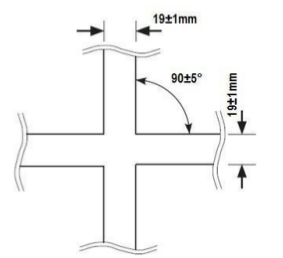
\includegraphics[scale=0.6]{figuras/Percurso1.png}
 \caption{Intersecções no percurso \label{fig:percurso1}}
 \vspace{-0.7cm}
 \caption*{Fonte: Disponível em \cite[p.4]{RegrasRobocore}.}
\end{figure}
%\captionsetup{width=0.50\textwidth, font=footnotesize, textfont=bf}






%A área que se estende entre o ponto de partida e o ponto de chegada, considerando 200mm da linha e 200mm a esquerda da linha
% é denominada ``área de partida-chegada'', conforme pode ser visto na Figura \ref{fig:percurso2}.\par
 A área que se estende entre o ponto de partida e o ponto de chegada, considerando 200mm a direita da linha e 
 200mm a esquerda da linha
 é denominada ``área de partida-chegada'', conforme pode ser visto na Figura \ref{fig:percurso2}.\par
 

\vspace{0.6cm}
\begin{figure}[h!]
 \centering
 \captionsetup{width=0.55\textwidth,font=footnotesize,textfont=bf}
 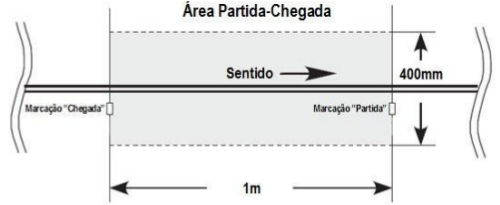
\includegraphics[scale=0.5]{figuras/Percurso2.png}
 \caption{Área de partida-chegada \label{fig:percurso2}}
  \vspace{-0.3cm}
 \caption*{Fonte: Disponível em \cite[p.4]{RegrasRobocore}.}
\end{figure}



%\captionsetup{width=0.50\textwidth, font=footnotesize, textfont=bf}
Quando houver um arco (intersecção entre a faixa branca), o raio deste é de pelo menos 100mm. Quando houver uma 
alteração na curvatura do percurso, deve haver uma marcação no lado esquerdo da linha, como pode ser visto na Figura 
\ref{fig:percurso4}.\par

\begin{figure}[t!]
 \centering
 \captionsetup{width=0.68\textwidth,font=footnotesize,textfont=bf}
 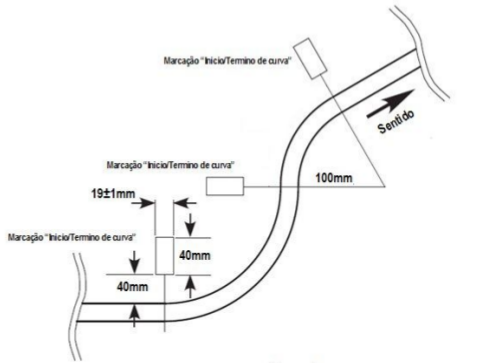
\includegraphics[scale=0.6]{figuras/Percurso4.png}
 \caption{Marcações de sinalização de curvatura \label{fig:percurso4}}
 \vspace{-0.3cm}
 \caption*{Fonte: Disponível em \cite[p.4]{RegrasRobocore}.}
\end{figure}


















